\documentclass[12pt,a4paper,oneside]{article}

\usepackage[absolute,overlay]{textpos}
\usepackage{graphicx}
\usepackage{adjustbox}
\usepackage{chemfig}
\usepackage[version=4]{mhchem}
\usepackage{wrapfig}
\usepackage{multirow}
\adjustboxset*{center}
\usepackage{subcaption}
\usepackage{chemformula}
\usepackage{elements}
\usepackage{hyperref}

\usepackage{parskip}

%dělení slov
\usepackage{ragged2e}
\let\raggedright=\RaggedRight
%konec dělení slov

\usepackage{fontspec}
\usepackage{unicode-math}

\usepackage{titlesec}
\titleformat{\chapter}[display]
{\normalfont\bfseries}{}{0pt}{\Large}

\usepackage{vcell}

\usepackage{polyglossia}
\setdefaultlanguage{czech}

\def\uv#1{„#1“}

\begin{document}

\title{Poznámky k seminářům z obecné chemie}
\author{Zdeněk Moravec, hugo@chemi.muni.cz}

\maketitle

\newpage
\setcounter{tocdepth}{2}
\tableofcontents

%\documentclass[hyperref=unicode, presentation,10pt]{beamer}

\usepackage[absolute,overlay]{textpos}
\usepackage{array}
\usepackage{graphicx}
\usepackage{adjustbox}
\usepackage{mhchem}
\usepackage{chemfig}
\usepackage{fontspec}
\usepackage[utf8]{inputenc}
\usepackage{caption}

%dělení slov
\usepackage{ragged2e}
\let\raggedright=\RaggedRight
%konec dělení slov

\addtobeamertemplate{frametitle}{
	\let\insertframetitle\insertsectionhead}{}
\addtobeamertemplate{frametitle}{
	\let\insertframesubtitle\insertsubsectionhead}{}

\makeatletter
\CheckCommand*\beamer@checkframetitle{\@ifnextchar\bgroup\beamer@inlineframetitle{}}
\renewcommand*\beamer@checkframetitle{\global\let\beamer@frametitle\relax\@ifnextchar\bgroup\beamer@inlineframetitle{}}
\makeatother
\setbeamercolor{section in toc}{fg=red}
\setbeamertemplate{section in toc shaded}[default][100]

\usepackage{fontspec}
\usepackage{unicode-math}

\usepackage{polyglossia}
\setdefaultlanguage{czech}

\def\uv#1{„#1“}

\mode<presentation>{\usetheme{default}}
 \usecolortheme{crane}

\setbeamertemplate{footline}[frame number]

\title[Crisis]
{Názvosloví}

\subtitle{Prvky, kyseliny, soli, komplexní sloučeniny}
%\author{\href{http://z-moravec.net/chemie/zaklady-chemie/}{http://z-moravec.net/}}
\author{Zdeněk Moravec, hugo@chemi.muni.cz}
\date{}

\begin{document}

\frame{\titlepage}

\section{Prvky}
\frame{
	\frametitle{}
	\vfill
	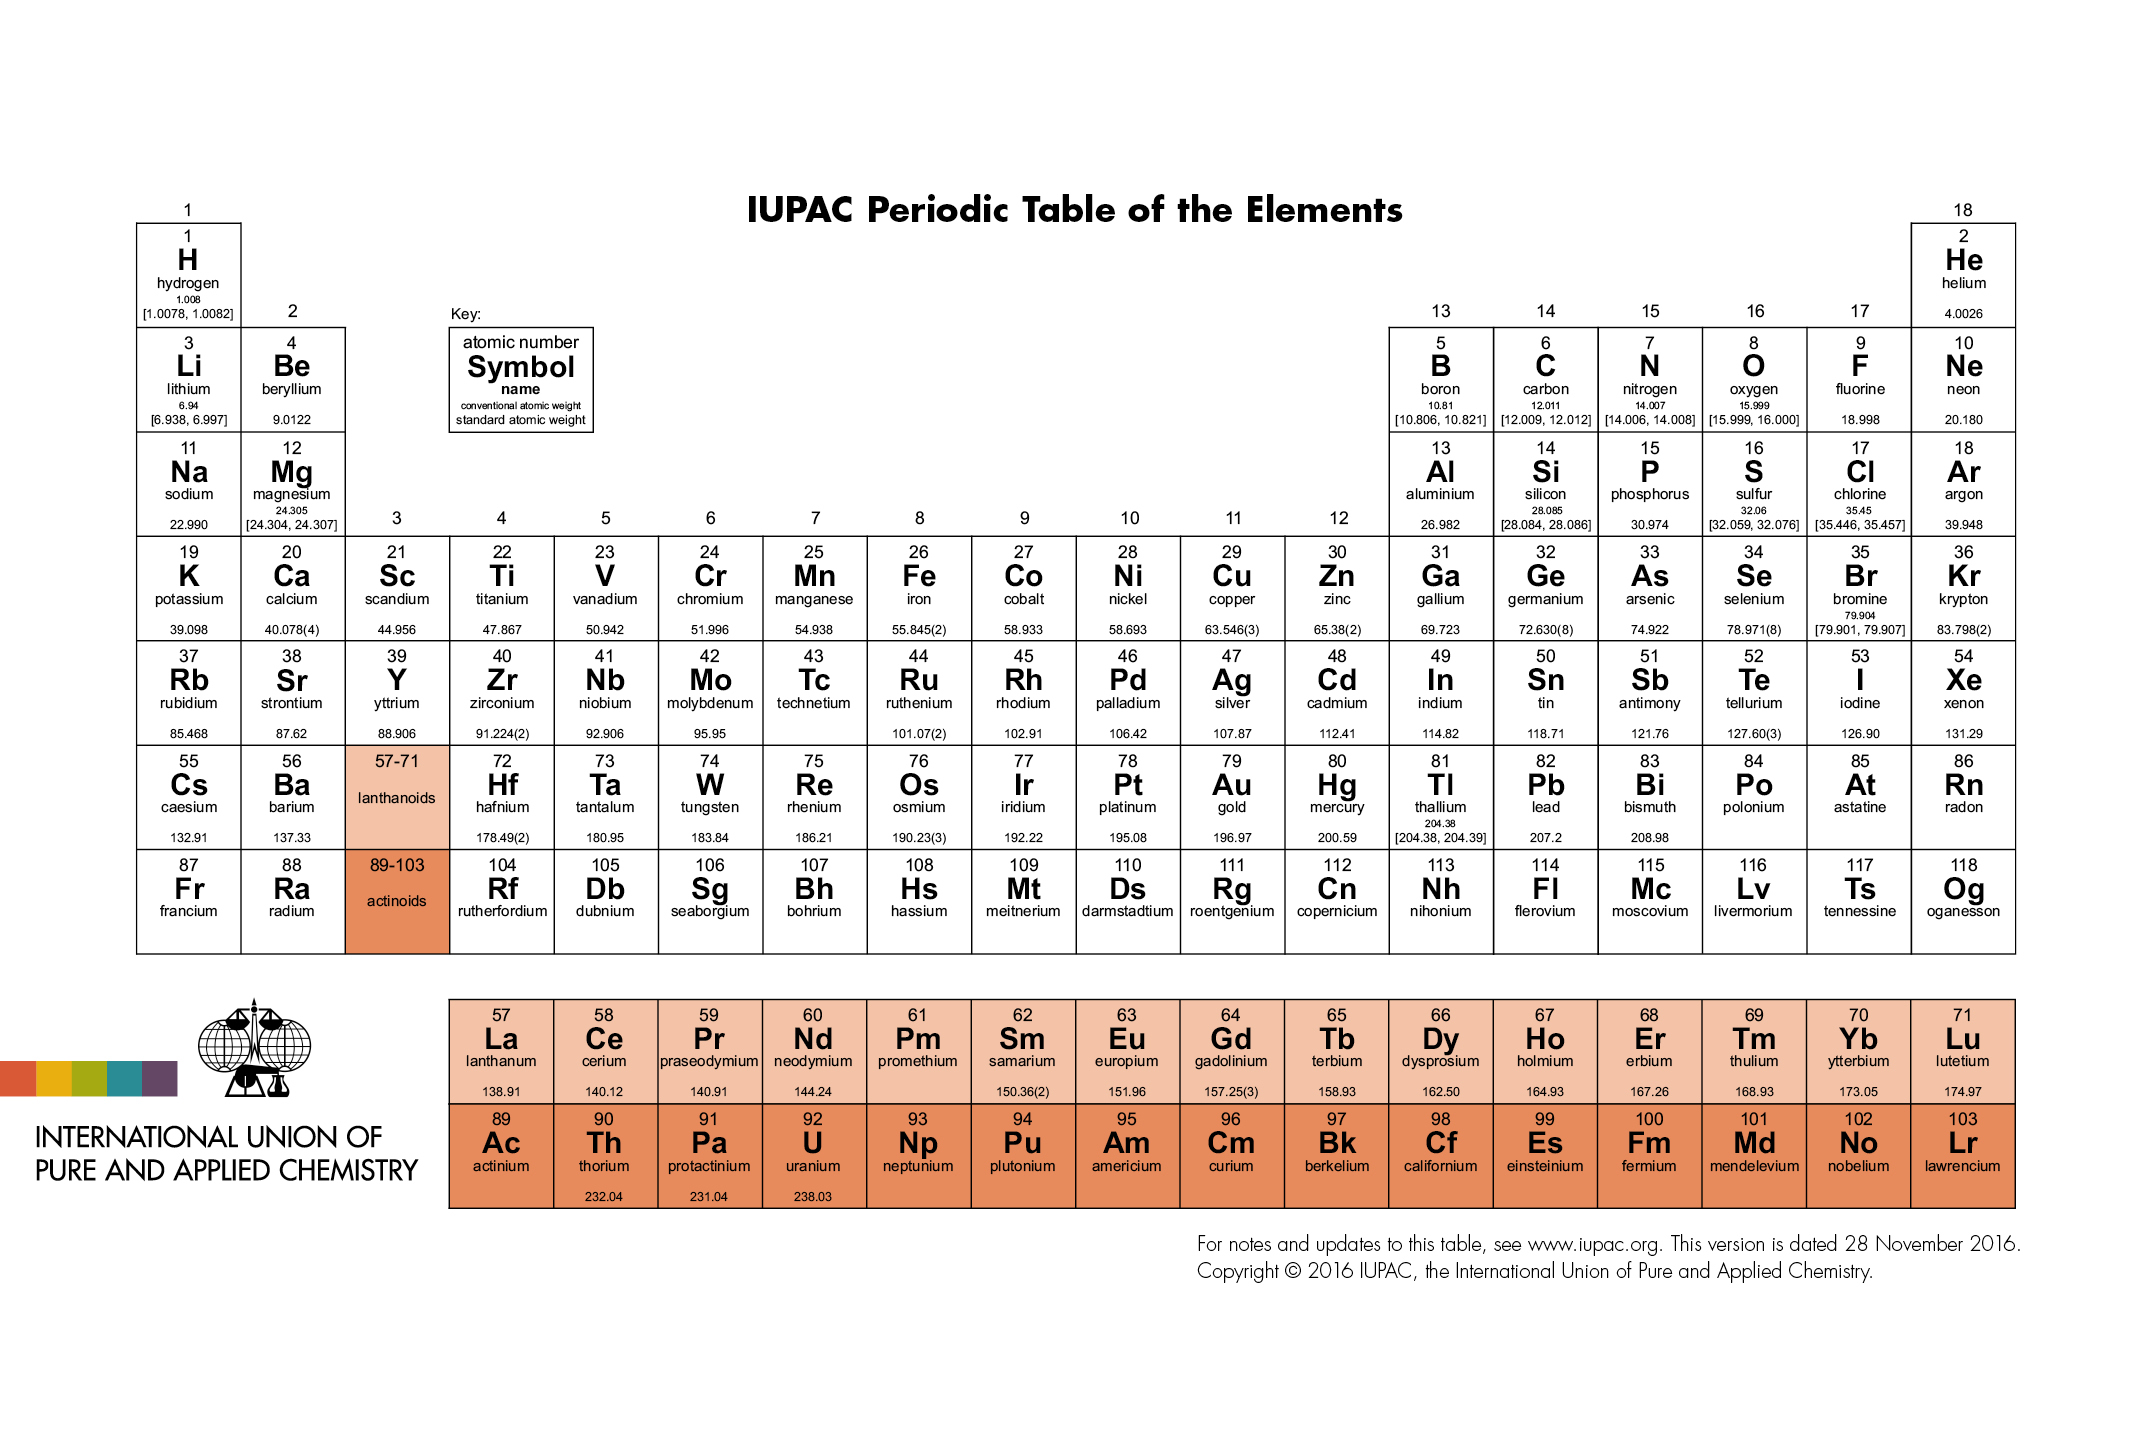
\includegraphics[keepaspectratio,width=1.1\textwidth]{PSP.png}
	\vfill
}

\frame{
	\frametitle{}
	\vfill
	\begin{tabular}{|ll|ll|ll|}
	\hline
	Bohrium & Bh & Curium & Cm & Darmstadtium & Ds \\\hline
	Einsteinium & Es & Flerovium & Fl & Hassium & Hs \\\hline
	Kalifornium & Cf & Kopernicium & Cn & Livermorium & Lv \\\hline
	Lutecium & Lu & Meitnerium & Mt & Promethium & Pm \\\hline
	Rhenium & Re & Rhodium & Rh & Roentgenium & Rg \\\hline
	Ruthenium & Ru & Rutherforium & Rf & Seaborgium & Sg \\\hline
	Tellur & Te & Thallium & Tl & Thulium & Tm \\\hline
	Ytterbium & Yb & Yttrium & Y & Tennessin & Ts \\\hline
	\end{tabular}
	\\[20pt]
	\begin{tabular}{|c|c|c|c|}
	\hline
	\multicolumn{4}{|c|}{\textbf{Nové prvky 7. periody}}\\\hline
	\textbf{Protonové číslo} & \textbf{Symbol} & \textbf{Český název} & \textbf{Latinský název} \\\hline
	113 & Nh & Nihonium & Nihonium \\\hline
	114 & Fl & Flerovium & Flerovium \\\hline
	115 & Mc & Moskovium & Moscovium \\\hline
	116 & Lv & Livermorium & Livermorium \\\hline
	117 & Ts & Tennessin & Tennessine \\\hline
	118 & Og & Oganesson & Oganesson  \\\hline
	\end{tabular}
	\vfill
}

\subsection{Skupiny prvků}
\frame{
	\frametitle{}
	\vfill
	\begin{tabular}{|l|l|l|l|l|}
		\hline
		\multicolumn{2}{|c|}{\textbf{Skupina}} & \textbf{Označení} & \textbf{Blok} & \textbf{Prvky} \\\hline
		1 & IA & Alkalické kovy & s & H, Li, Na, K, Rb, Cs, Fr \\\hline
		2 & IIA & Kovy alkalických zemin & s & Be, Mg, Ca, Sr, Ba, Ra \\\hline
		3 & IIIB &  & d & Sc, Y, La, Ac \\\hline
		4 & IVB &  & d & Ti, Zr, Hf, Rf \\\hline
		5 & VB &  & d & V, Nb, Ta, Db \\\hline
		6 & VIB &  & d & Cr, Mo, W, Sg \\\hline
		7 & VIIB &  & d & Mn, Tc, Re, Bh \\\hline
		8 & VIIIB &  & d & Fe, Ru, Os, Hs \\\hline
		9 & VIIIB &  & d & Co, Rh, Ir, Mt \\\hline
		10 & VIIIB &  & d & Ni, Pd, Pt, Ds \\\hline
		11 & IB &  & d & Cu, Ag, Au, Rg \\\hline
		12 & IIB &  & d & Zn, Cd, Hg, Cn \\\hline
	\end{tabular}
	\vfill
}

\frame{
	\frametitle{}
	\vfill
	\begin{tabular}{|l|l|l|l|l|}
		\hline
		\multicolumn{2}{|c|}{\textbf{Skupina}} & \textbf{Označení} & \textbf{Blok} & \textbf{Prvky} \\\hline
		13 & IIIA & Triely & p & B, Al, Ga, In, Tl, Nh \\\hline
		14 & IVA & Tetrely & p & C, Si, Ge, Sn, Pb, Fl \\\hline
		15 & VA & Pentely & p & N, P, As, Sb, Bi, Mc \\\hline
		16 & VIA & Chalkogeny & p & O, S, Se, Te, Po, Lv \\\hline
		17 & VIIA & Halogeny & p & F, Cl, Br, I, At, Ts \\\hline
		18 & VIIIA & Vzácné plyny & p & He, Ne, Xe, Ar, Kr, Xe, Rn, Og \\\hline
	\end{tabular}
	\vfill
}

\frame{
	\frametitle{}
	\vfill
	\begin{itemize}
		\item \textbf{Lanthanoidy} -- Ce, Pr, Nd, Pm, Sm, Eu, Gd, Tb, Dy, Ho, Er, Tm, Yb, Lu
		\item \textbf{Aktinoidy} -- Th, Pa, U, Np, Pu, Am, Cm, Bk, Cf, Es, Fm, Md, No, Lr
		\item \textbf{Transurany} -- Np, Pu, Am, Cm, Bk, Cf, Es, Fm, Md, No, Lr, transaktinoidy
		\item \textbf{Transaktinoidy} -- Rf, Db, Sg, Bh, Hs, Mt, Ds, Rg, Cn, Nh, Fl, Mc, Lv, Ts, Og
		\item \textbf{Vzácné zeminy} -- Sc, Y, La, Ce, Pr, Nd, Pm, Sm, Eu, Gd, Tb, Dy, Ho, Er, Tm, Yb, Lu
		\item \textbf{Skupina železa} -- Fe, Co, Ni
		\item \textbf{Lehké Pt kovy} -- Ru, Rh, Pd
		\item \textbf{Těžké Pt kovy} -- Os, Ir, Pt
	\end{itemize}
	\vfill
}

\section{Předpony a přípony}
\frame{
	\frametitle{}
	\begin{columns}
	\column{.6\textwidth}
	\begin{tabular}{|l|l|l|l|}
	\hline
	\parbox[t]{1.5cm}{Oxidační \\ číslo} & Kation & Sůl & Kyselina \\\hline
	I & -ný & -nan & -ná \\\hline
	II & -natý & -natan & -natá \\\hline
	III & -itý & -itan & -itá \\\hline
	IV & -ičitý & -ičitan & -ičitá \\\hline
	V & \parbox[t]{1cm}{-ičný \\ -ečný} &  \parbox[t]{1.2cm}{-ičnan \\ -ečnan} &  \parbox[t]{1cm}{-ičná \\ -ečná} \\\hline
	VI & -ový & -an & -ová \\\hline
	VII & -istý & -istan & -istá \\\hline
	VIII & -ičelý & -ičelan & -ičelá \\\hline
	\end{tabular}

	\column{.4\textwidth}
	\begin{tabular}{|l|l|}
	\hline
	Číslovka & Předpona \\\hline
	$^1/_2$ & hemi- \\\hline
	1 & mono- \\\hline
	2 & di- \\\hline
	3 & tri- \\\hline
	4 & tetra- \\\hline
	5 & penta- \\\hline
	6 & hexa- \\\hline
	7 & hepta- \\\hline
	8 & okta- \\\hline
	9 & nona- \\\hline
	10 & deka- \\\hline
	11 & undeka- \\\hline
	12 & dodeka- \\\hline
	\end{tabular}
	\end{columns}
}

\section{Oxidační číslo}
\frame{
	\frametitle{}
	\begin{itemize}
	\item Oxidační číslo je formální náboj, který by atom měl, pokud bychom všechny vazebné elektrony přisoudili elektronegativnějšímu prvku.
	\item Součet oxidačních čísel všech atomů molekuly je roven nule.
	\item Součet oxidačních čísel všech atomů iontu je roven jeho náboji (vč. znaménka).
	\item \textbf{Vodík} se ve sloučeninách vyskytuje nejčastěji v oxidačním stavu I, výjimkou jsou hydridy, kde má oxidační číslo -I. V hydridech nekovů má vodík konvenčně oxidační číslo I.
	\begin{itemize}
	\item \ce{H2^IO^{-II}}: $2\times 1+(-2) = 0$ - voda (oxan)
	\item \ce{Ca^{II}H2^{-I}}: $2+2\times(-1) = 0$ - hydrid vápenatý
	\end{itemize}
	\item \textbf{Kyslík} tvoří sloučeniny ve třech oxidačních stavech
	\begin{itemize}
	\item Oxidy: \ce{K2^IO^{-II}}: $2\times1+(-2) = 0$ - oxid draselný
	\item Peroxidy \ce{K2^{I}O2^{-I}}: $2\times1+2\times(-1) = 0$ - peroxid draselný
	\item Hyperoxidy \ce{K^{I}O2^{-1/2}}: $1+2\times(-\frac{1}{2}) = 0$ - hyperoxid draselný
	\end{itemize}
	\item \ce{(S^{VI}O4^{-II})^{2-}}: $6 + 4\times(-2) = -2$ - síran
	\item \ce{(Cl^{VII}O4^{-II})^{-}}: $7 + 4\times(-2) = -1$ - chloristan
	\end{itemize}
}

\section{Kyseliny a soli}
\frame{
	\frametitle{}
	\begin{tabular}{lll}
	\ce{H2SO4} & \ce{H2^IS^{VI}O4^{-II}} & kyselina sírová \\
	\ce{Na2SO4} & \ce{Na2^IS^{VI}O4^{-II}} & síran sodný \\
	\ce{H3PO4} & \ce{H3^IP^{V}O4^{-II}} & kyselina trihydrogenfosforečná \\
	\ce{Na3PO4} & \ce{Na3^IP^{V}O4^{-II}} & fosforečnan sodný \\
	\ce{Na2HPO4} & \ce{Na2^IH^IP^{V}O4^{-II}} & hydrogenfosfo\-rečnan sodný \\
	\ce{NaH2PO4} & \ce{Na^IH2^IP^{V}O4^{-II}} & dihydrogenfosfo\-rečnan sodný \\
	\ce{CaH2} & \ce{Ca^{II}H2^{-I}} & hydrid vápenatý \\
	\ce{AlH3} & \ce{Al^{III}H3^{-I}} & alan (hydrid hlinitý) \\
	\ce{SeH2} & \ce{Se^{II}H2^{-I}} & selan \\
	\ce{PH3} & \ce{P^{-III}H3^{I}} & fosfan \\
	\ce{PH5} & \ce{P^{-V}H5^{I}} & fosforan \\
	\ce{H2O2} & \ce{H2^IO2^{-I}} & peroxid vodíku \\
	\ce{NaNO2.10H2O} & \ce{Na^IN^{III}O2^{-II}.10H2O} & dekahydrát dusitanu sodného \\
	\ce{Al2S3} & \ce{Al2^{III}S3^{-II}} & sulfid hlinitý \\
	\ce{KCN} & \ce{K^IC^{II}N^{-III}} & kyanid draselný \\
	\end{tabular}
}

\subsection{Podvojné soli}
\frame{
	\frametitle{}
	\begin{itemize}
		\item Ve vzorcích podvojných solí se kationty uvádějí v pořadí rostoucích oxidačních čísel, v případě stejného oxidačního čísla v abecedním pořadí.
		\item Víceatomové kationty, např. \ce{NH$_4^+$} nebo \ce{PH$_4^+$} se uvádějí poslední.
		\item V názvu se oddělují pomlčkou a pořadí je dáno pořadím ve vzorci.
		\item \ce{K2NH4PO4} -- fosforečnan didraselno-amonný
		\item \ce{NH4MgPO4} -- fosforečnan amonno-hořečnatý
		\item \ce{NaNH4SO4} -- síran sodno-amonný
		\item Anionty se uvádějí v abecedním pořadí značek prvků, příp. centrálních atomů.
		\item \ce{Ca3(CO3)2F2} -- bis(uhličitan)-difluorid trivápenatý
		\item \ce{Na6ClF(SO4)2} -- chlorid-fluorid-bis(síran) hexasodný
		\item Podvojné oxidy je nutné pojmenovávat jako oxidy, ne jako soli. Jedinou výjimkou jsou situace, kdy je prokázáno, že sloučenina obsahuje daný anion, např. \ce{TiO$_3^{2-}$}:
		\item \ce{FeTiO3} -- trioxid železnato-titaničitý
		\item \ce{NaNbO3} -- trioxid sodno-niobičný
	\end{itemize}
}

\section{Názvy iontů}
\frame{
	\frametitle{}
	\begin{itemize}
	\item Názvy jednoatomových kationtů mají koncovku danou oxidačním číslem kovu.
	\item Názvy jednoatomových aniontů mají koncovku \textbf{-id}.
	\item U víceatomových kationtů používáme koncovku \textbf{-onium}.
	\item Názvy aniontů odvozených od kyslíkatých kyselin se tvoří tak, že se v koncovce dané oxidačním číslem (např. -itý) zamění \textbf{-ý} za \textbf{-an}.
	\end{itemize}
	\begin{tabular}{llll}
	\ce{Cl^-} & chlorid & \ce{NaCl} & chlorid sodný \\
	$\textrm{NH}_2^-$ & amid & \ce{NaNH2} & amid sodný \\
	\ce{N^{3-}} & nitrid & \ce{Hg3N2} & nitrid rtuťnatý \\
	\ce{C^{4-}} & karbid & \ce{Al4C3} & karbid hlinitý \\
	$\textrm{SO}_{4}^{2-}$ & síran & \ce{K2SO4} & síran draselný \\
	$\textrm{PH}_4^+$ & fosfonium & \ce{PH4Cl} & chlorid fosfonia \\
	$\textrm{H}_2\textrm{NO}_3^+$ & nitratacidium & \ce{(H2NO3)_2SO4} & síran nitratacidia \\
	\ce{[(CH3)3NH]^+} & trimethylamonium & \ce{[(CH3)3NH]Br} & \parbox{2cm}{bromid \\trimethylamonia} \\
	\end{tabular}
}

\subsection{Ionty odvozené od amoniaku}
\frame{
	\frametitle{}
	\begin{itemize}
		\item Z amoniaku můžeme odvodit \textit{amonný kation}, \ce{NH$_4^+$}.
		\item \ce{(NH4)2SO4} -- síran amonný
		\item \ce{Na(NH4)SO4} -- síran sodno-amonný
		\item \ce{(NH4)Al(SO4)2.12H2O} -- dodekahydrát síranu amonno-hlinitého
		\item Substitucí protonů získáme alkylamonné soli.
		\item \ce{(NMe4)2SO4} -- síran tetramethylamonný
		\item \ce{NH2Me2Br} -- bromid dimethylamonný
	\end{itemize}
	\begin{figure}
		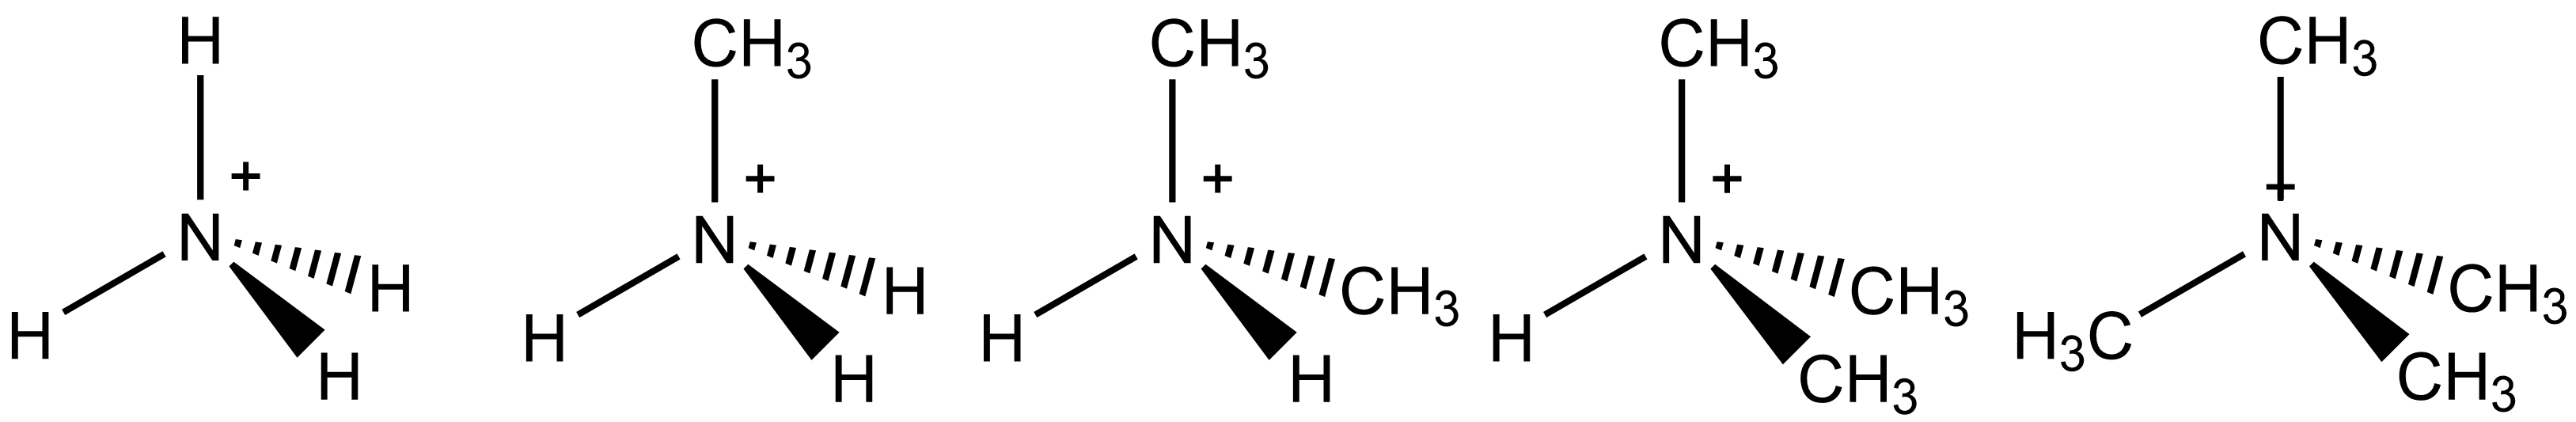
\includegraphics[width=\textwidth]{NH4.png}
		\caption*{Kationty amonný, methylamonný, dimethylamonný, trimethylamonný a tetramethylamonný}
	\end{figure}
}

\frame{
	\frametitle{}
	\begin{itemize}
		\item Postupným odštěpováním protonů z \ce{NH3} získáme tři anionty:
		\begin{itemize}
			\item \ce{NH$_2^-$} -- amid
			\item \ce{NH^{2-}} -- imid
			\item \ce{N^{3-}} -- nitrid
		\end{itemize}
	\end{itemize}

	\begin{tabular}{|l|l||l|l|}
		\hline
		\ce{LiNH2} & amid lithný & \ce{Si(NH2)4} & amid křemičitý \\\hline
		\ce{Li2NH} & imid lithný & \ce{CaNH} & imid vápenatý \\\hline
		\ce{Li3N} & nitrid lithný & \ce{CO(NH2)2} & amid kyseliny uhličité \\\hline
		\ce{AlN} & nitrid hlinitý & \ce{SO2(NH2)2} & amid kyseliny sírové \\\hline
		\ce{Ti3N4} & nitrid titaničitý & \ce{SO(NH2)2} & amid kyseliny siřičité \\\hline
	\end{tabular}
	\begin{figure}
		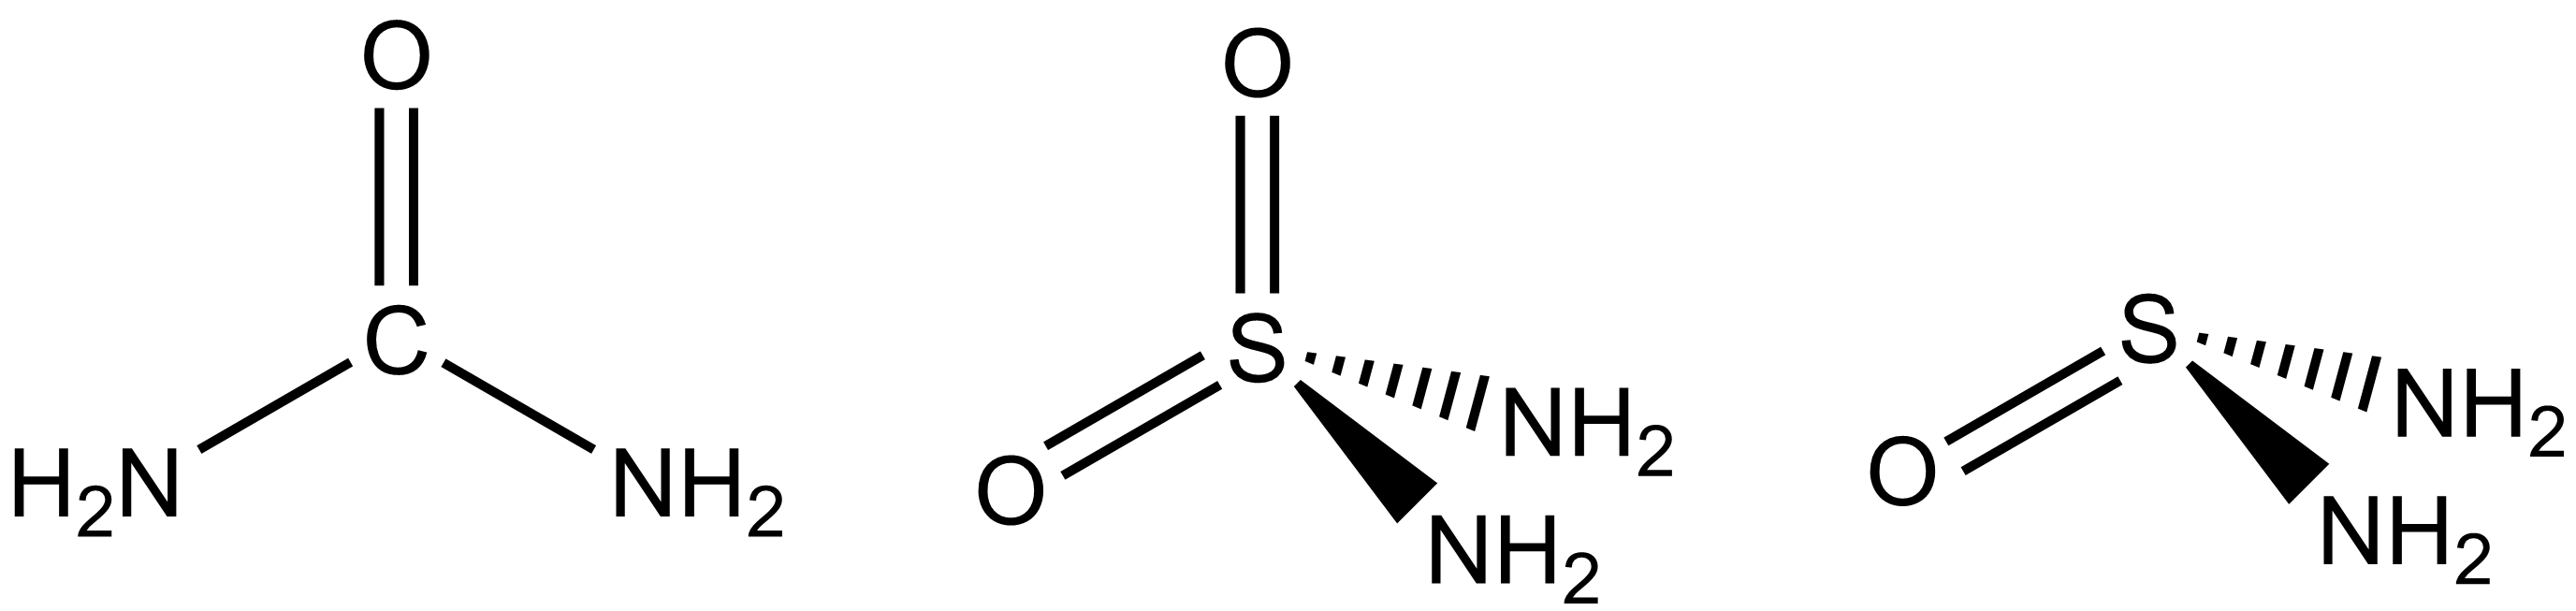
\includegraphics[width=\textwidth]{amides.png}
	\end{figure}
}

\section{Atomové skupiny}
\frame{
	Názvy atomových skupin končí, nezávisle na jejich náboji, koncovkou \textbf{-yl}. Pokud existuje více skupin stejného složení, ale lišící se nábojem, rozlišujeme je uvedením náboje nebo oxidačního čísla centrálního atomu v názvu.
\\
	\begin{tabular}{llllll}
	\ce{OH} & hydroxyl & \ce{CO} & karbonyl & \ce{NO} & nitrosyl \\
	\ce{NO2} & nitryl & \ce{PO} & fosforyl & \ce{VO} & vanadyl \\
	\ce{SO} & thionyl & \ce{SO2} & sulfuryl & \ce{SeO} & seleninyl \\
	\ce{SeO2} & selenonyl & \ce{CrO2} & chromyl & \ce{UO2} & uranyl \\
	\ce{ClO} & chlorosyl & \ce{ClO2} & chloryl & \ce{ClO3} & perchloryl \\
	\end{tabular}
	\newline
	\newline
	\newline
	\ce{COCl2} - chlorid karbonylu \\
	\ce{SO2Cl2} - chlorid sulfurylu \\
	\ce{UO2(NO3)2} - dusičnan uranylu(2+) nebo dusičnan uranylu(VI)
}

\section{Atomové skupiny}
\frame{
	Názvy atomových skupin končí, nezávisle na jejich náboji, koncovkou \textbf{-yl}. Pokud existuje více skupin stejného složení, ale lišící se nábojem, rozlišujeme je uvedením náboje nebo oxidačního čísla centrálního atomu v názvu.
	\\
	\begin{tabular}{llllll}
		\ce{OH} & hydroxyl & \ce{CO} & karbonyl & \ce{NO} & nitrosyl \\
		\ce{NO2} & nitryl & \ce{PO} & fosforyl & \ce{VO} & vanadyl \\
		\ce{SO} & thionyl & \ce{SO2} & sulfuryl & \ce{SeO} & seleninyl \\
		\ce{SeO2} & selenonyl & \ce{CrO2} & chromyl & \ce{UO2} & uranyl \\
		\ce{ClO} & chlorosyl & \ce{ClO2} & chloryl & \ce{ClO3} & perchloryl \\
	\end{tabular}
	\newline
	\newline
	\newline
	\ce{COCl2} - chlorid karbonylu \\
	\ce{UO2(NO3)2} - dusičnan uranylu(2+) nebo dusičnan uranylu(VI)
}

\section{Estery anorganických kyselin}
\frame{
	\begin{figure}
		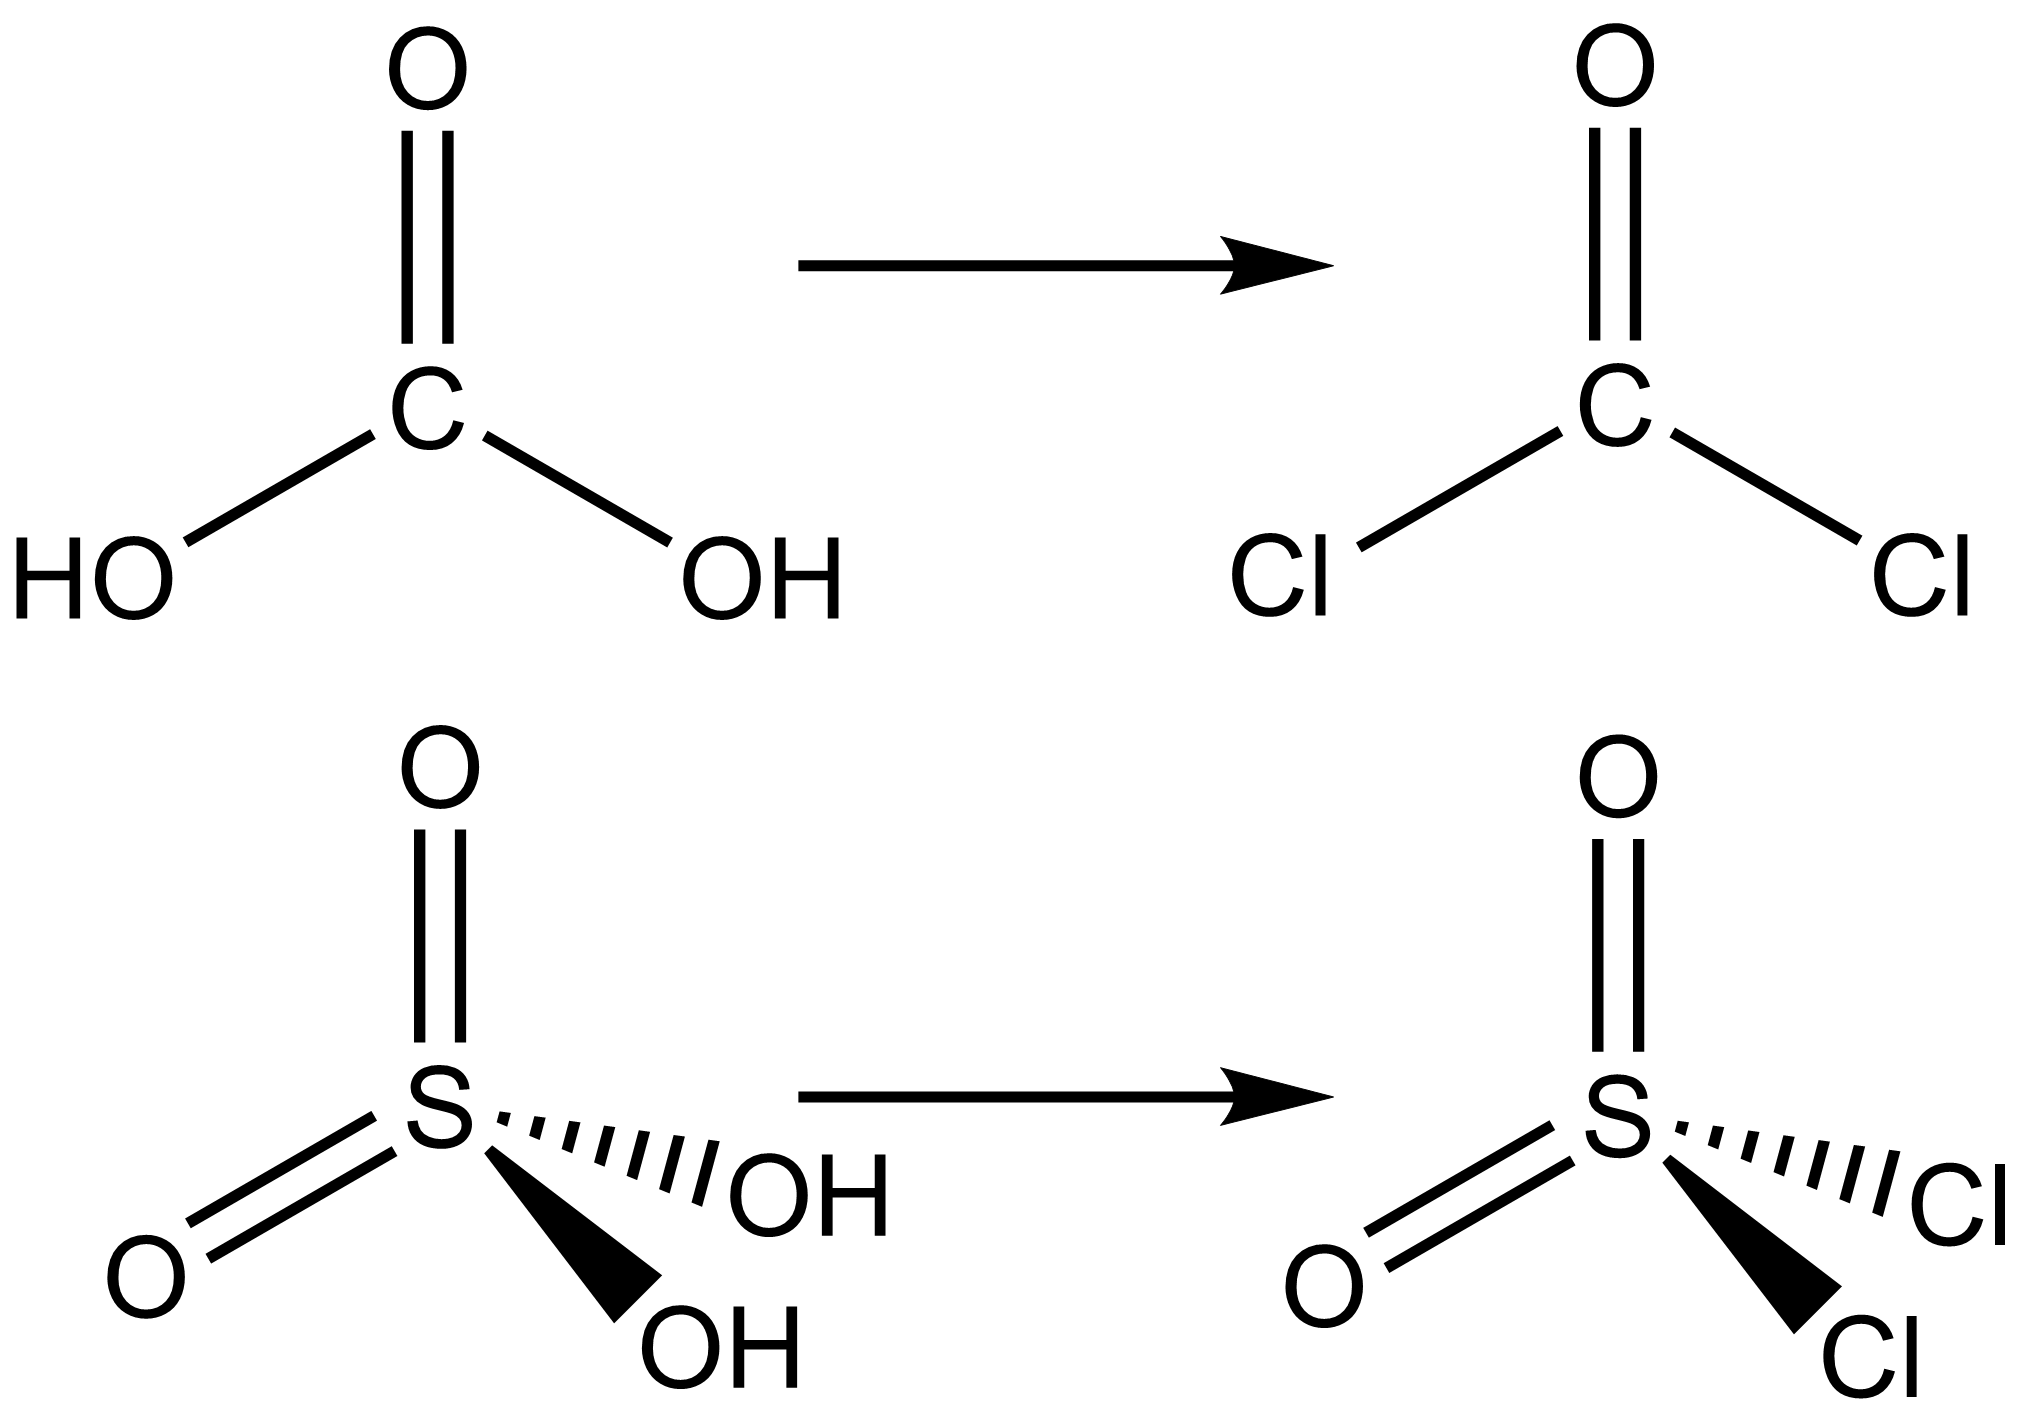
\includegraphics[keepaspectratio,width=\textwidth]{estery.png}
	\end{figure}
}

\section{Izo- a heteropolyanionty}
\frame{
	\frametitle{}
	\begin{itemize}
	\item \textbf{Izopolyanionty} jsou anionty obsahující dva a více centrálních atomů téhož prvku.
	\item \textbf{Heteropolyanionty} jsou anionty obsahující dva a více centrálních atomů různých prvků.
	\item Vznikají kondenzací monomerních jednotek, např.:
	\begin{itemize}
	\item \ce{2 K2CrO4 + 2 HCl -> K2Cr2O7 + H2O + 2 KCl}
	\item \chemfig{O^{\ominus}-Cr(=[2]O)(=[6]O)-O-Cr(=[2]O)(=[6]O)-O^{\ominus}}
	\end{itemize}
	\item Cyklické a řetězovité struktury odlišujeme předponami cyklo- a katena-.
	\item U heteropolyaniontů se názvy jednotlivých složek řadí v pořadí, v jakém jsou zapsány ve vzorci a oddělují se pomlčkami. Pořadí volíme tak, abychom začínali kovem, jehož značka je v abecedním pořadí co nejblíže začátku.
	\begin{itemize}
	\item \ce{(O3CrOAsO2OPO3)^{4-}} - anion chromano-arseničnano-fosforečnanový(4-)
	\end{itemize}
	\end{itemize}
}

\section{Koordinační sloučeniny}
\frame{
	\frametitle{}

	Koordinační sloučenina je sloučenina obsahující alespoň jednu donor-akceptorovou vazbu.
	Název těchto sloučenin se tvoří pojmenováním centrálního atomu a jednotlivých ligandů.
	\newline
	\newline

	\begin{tabular}{lll}
	\textbf{Vzorec} & \textbf{Ion} & \textbf{Ligand} \\
	\ce{SO$_4^{2-}$} & Síran & Sulfato- \\
	\ce{S2O$_3^{2-}$} & Thiosíran & Thiosulfato- \\
	\ce{PO$_4^{3-}$} & Fosforečnan & Fosfato- \\
	\ce{CH3COO^{-}} & Octan & Acetato- \\
	\ce{F^{-}} & Fluorid & Fluoro- \\
	\ce{O^{2-}} & Oxid & Oxido- \\
	\ce{H^{-}} & Hydrid & Hydrido- \\
	\ce{SCN^{-}} & Thiokyanatan & Thiokyanato- \\
	\end{tabular}
}

\subsection{Organické ligandy}
\frame{
	\frametitle{}

	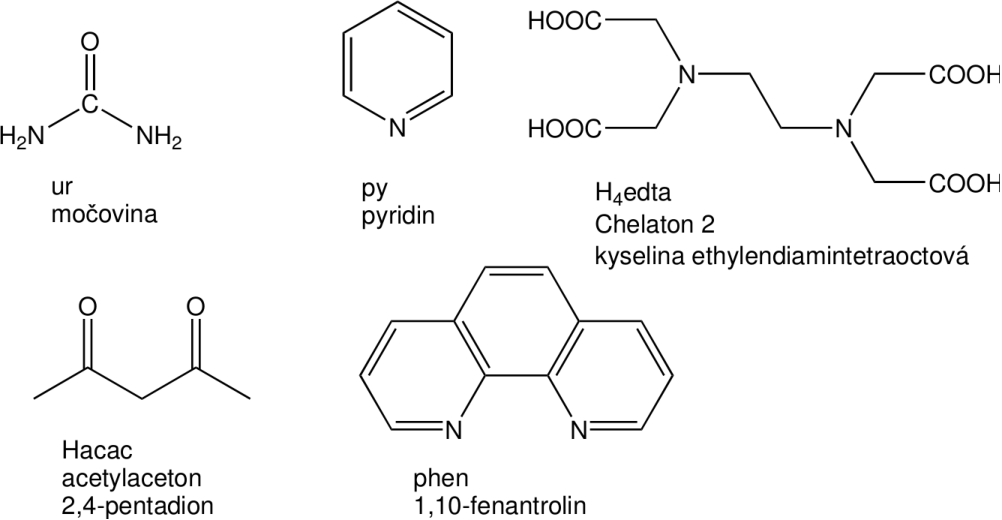
\includegraphics[keepaspectratio,width=105mm]{ligandy.pdf}
}

\subsection{Izomerie}
\frame{
	\frametitle{}

	a) Ligand se koordinuje k centrálnímu atomu různými donorovými atomy. Jev se nazývá \textbf{vazebná izomerie} a izomery rozlišujeme rozdílnými názvy ligandů
\vspace{5mm}
\\
\begin{tabular}{llll}
\ce{-NO2} & nitro & \ce{-ONO} & nitrito \\
\ce{-SCN} & thiokyanato & \ce{-NCS} & isothiokyanato \\
\ce{-SeCN} & selenokyanato & \ce{-NCSe} & isoselenokyanato \\
\end{tabular}
\\
\vspace{10mm}
b) Koordinují se izomerní ligandy za vzniku \textbf{polohových izomerů}. I tento případ se vystihne rozdílným názvem ligandů
\vspace{5mm}
\\
\begin{tabular}{ll}
\textcolor{red}{H$_2$N}CH$_2$CH(\textcolor{red}{NH$_2$})CH$_3$ & 1,2-diaminopropan \\
CH$_3$\textcolor{red}{NH}CH$_2$CH$_2$\textcolor{red}{NH$_2$} & N-methylethylendiamin \\
\end{tabular}
}

\frame{
	\frametitle{}
c) Komplex má zaměněny ionty v koordinační a iontové sféře. Tuto situaci, nazývanou \textbf{ionizační izomerie}, řeší název komplexu
\\
\vspace{1cm}
\begin{tabular}{ll}
\ce{[Co(NH3)5SO4]Br} & bromid pentaammin-sulfatokobaltitý \\
\ce{[Co(NH3)5Br]SO4} & síran pentaammin-bromokobaltitý  \\
\end{tabular}
\vspace{1cm}
\\
d) U koordinačních sloučenin s komplexním kationtem i aniontem se může měnit rozdělení ligandů mezi koordinačními sférami obou centrálních atomů (\textbf{koordinační izomerie}) \\
\vspace{1cm}
\begin{tabular}{ll}
\ce{[Pt(NH3)4][CuCl4]} & tetrachloroměďnatan tetramminplatnatý \\
\ce{[Cu(NH3)4][PtCl4]} & tetrachloroplatnatan tetraamminměďnatý \\
\end{tabular}
}

\frame{
	\frametitle{}

	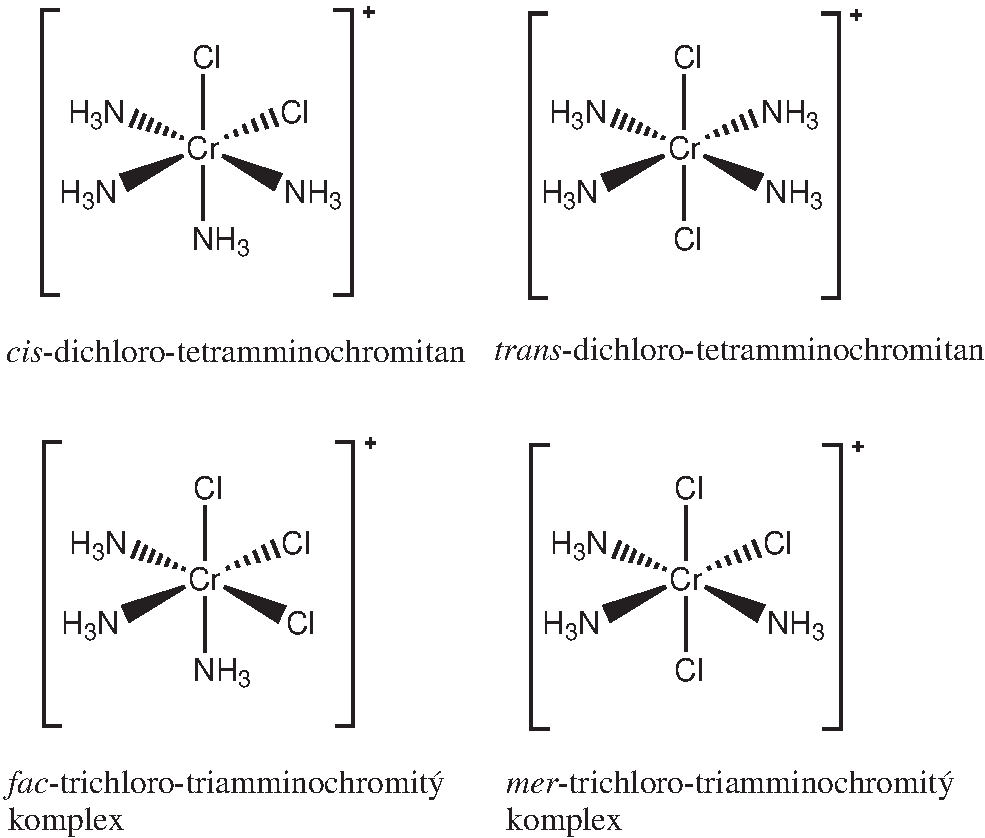
\includegraphics[keepaspectratio,width=100mm]{izomery.pdf}
}

\end{document}
%\newpage


\section{Platné číslice}

\textbf{Platné číslice} jsou číslice odečtené z měřící stupnice přístroje, vč. posledního odhadnutého místa.\footnote{\href{https://is.muni.cz/do/sci/UChem/um/laboratorni_technika/pages/uvod.html}{Chyby měření}}

Nuly mezi desetinnou čárkou a první nenulovou číslicí nejsou platné číslice:

\textbf{25,23} cm = \textbf{2523}00 $\mu$m = \textbf{2,523}$\times$10$^5$ $\mu$m

Platné jsou vždy čtyři číslice, vyznačený tučnou sazbou.

Při \textbf{sčítání a odečítání} má výsledek tolik \textit{desetinných míst} jako číslo s nejmenším počtem desetinných míst:

2,5 cm + 5,236 cm = 7,7 cm\\
2,5 cm + 3,3 $\mu$m = 2,5 cm

Při \textbf{násobení a dělení} má výsledek tolik \textit{platných číslic} jako číslo s nejmenším počtem platných číslic (platné číslice jsou vyznačeny tučně):

n = c . V = 0,0\textbf{50} . 0,0\textbf{1235} = 0,000\textbf{61}75 mol = 6,2$\times10^{-4}$ mol

\textbf{Při výpočtech se vždy zaokrouhluje až poslední výsledek. Zaokrouhlování mezivýpočtů zvyšuje chybu výpočtu.}
\newpage

%\include{02-stechiom-vzorec.tex}
%\newpage

\section{Termochemie}
\textbf{Vypočítejte reakční entalpii přeměny grafitu na diamant:}\\
\ce{C(gr) -> C(diam)}\\
jestliže znáte entalpie reakcí:\\
\begin{tabular}{clr@{,}l}
	A: & \ce{C(gr) + O2(g) -> CO2(g)} & $-$393 & 77 kJ.mol$^{-1}$ \\
	B: & \ce{C(diam) + O2(g) -> CO2(g)} & $-$395 & 65 kJ.mol$^{-1}$ \\
\end{tabular}
\\
Jelikož nás zajímá přeměna grafitu na diamant, vezmeme entalpii spalování grafitu a od ní odečteme entalpii spalování diamantu: \textbf{A$-$B}\\
\ce{C(gr) + O2(g) + CO2(g) -> C(diam) + O2(g) + CO2(g)}
\\
Entalpii tedy vypočítáme:\\
$\Delta H_r\ =\ -393,77\ -(-395,65)\ =\ 1,88$ kJ.mol$^{-1}$
\\
\textbf{Entalpie přeměny grafitu na diamant bude 1,88 kJ.mol$^{-1}$}\\
\hrule

\textbf{Vypočítejte entalpii spalování acetylenu:}\\
\ce{C2H2(g) + \frac{5}{2} O2(g) -> 2 CO2(g) + H2O(l)}\\
jestliže znáte entalpie reakcí:\\
\begin{tabular}{clr@{,}l}
	A: & \ce{2 C(s) + H2(g) -> C2H2(g)} & 226 & 92 kJ.mol$^{-1}$ \\
	B: & \ce{2 C(s) + O2(g) -> CO2(g)} & $-$393 & 97 kJ.mol$^{-1}$ \\
	C: & \ce{H2(g) + \frac{1}{2} O2(g) -> H2O(l)} & $-$285 & 96 kJ.mol$^{-1}$ \\
\end{tabular}

Zadanou rovnici získáme následující kombinací známých reakcí:\\
$-$A+2B+C\\
Entalpii tedy vypočítáme:\\
$\Delta H_r\ =\ -226,92\ -\ 2.393,7\ - 285,96\ =\ -1300,82$ kJ.mol$^{-1}$\\
\textbf{Entalpie zadané reakce bude $-$1300,82 kJ.mol$^{-1}$}

\newpage

\documentclass[12pt,a4paper,oneside]{article}

\usepackage[absolute,overlay]{textpos}
\usepackage{graphicx}
\usepackage{adjustbox}
\usepackage{chemfig}
\usepackage[version=4]{mhchem}
\usepackage{wrapfig}
\usepackage{multirow}
\adjustboxset*{center}
\usepackage{caption}
\usepackage{chemformula}
\usepackage{elements}

%dělení slov
\usepackage{ragged2e}
\let\raggedright=\RaggedRight
%konec dělení slov

\usepackage{fontspec}
\usepackage{unicode-math}

\usepackage{polyglossia}
\setdefaultlanguage{czech}

\def\uv#1{„#1“}

\begin{document}

\section{pH}
\subsection{Vzorce}

\begin{tabular}{|l|l|}
	\hline
	Silná kyselina & pH = $-\log$c \\\hline
	Silná zásada & pH = 14 + $\log$c \\\hline
	Slabá kyselina & pH = $\frac{1}{2}\textrm{p}K_A-\frac{1}{2}\log$c \\[1em] \hline
	Slabá zásada & pH = $14\ +\ \frac{1}{2}\log\textrm{c} - \frac{1}{2}\textrm{p}K_B$ \\[1em] \hline
\end{tabular}
\end{document}
\newpage

\section{Krystaly}

V elementární buňce rozlišujeme čtyři typy poloh:
\begin{enumerate}
	\item Poloha uvnitř buňky, atom patří celý do jediné buňky
	\item Poloha ve středu stěny, atom je sdílen dvěma buňkami. V konkrétní buňce je umístěna polovina atomu.
	\item Poloha ve středu hrany, atom je sdílen čtyřmi buňkami. V konkrétní buňce je umístěna čtvrtina atomu.
	\item Poloha ve vrcholu buňky, atom je sdílen osmi buňkami. V konkrétní buňce je umístěna osmina atomu.
\end{enumerate}

\begin{figure}[h]
	\adjincludegraphics[width=.3\textwidth]{img/08-CsCl.png}
	\caption[Krystalová struktura chloridu cesného.]{Krystalová struktura chloridu cesného.\footnotemark}
\end{figure}
\footnotetext{Zdroj: \href{https://commons.wikimedia.org/wiki/File:Caesium-chloride-unit-cell-3D-balls.png}{Benjah-bmm27/Commons}}

Např. chlorid cesný obsahuje cesný ion ve středu kubické buňky a osm chloridových aniontů v jejích vrcholech. Cesný kation patři do krystalové buňky celý a každý chlorid tam spadá $\frac{1}{8}$, tzn. vzorec je CsCl$_{8\times\frac{1}{8}}$ = CsCl.

\begin{figure}[h]
	\adjincludegraphics[width=.3\textwidth]{img/08-TiO2.png}
	\caption[Krystalová struktura chloridu cesného.]{Krystalová struktura oxidu titaničitého.\footnotemark}
\end{figure}
\footnotetext{Zdroj: \href{https://commons.wikimedia.org/wiki/File:Kristallstruktur_Titandioxid.png}{Orci/Commons}}

\begin{enumerate}
	\item Ti: šedé, 8$\times\frac{1}{8}$ + 1 = 2
	\item O: červené, 2$\times$1 + 4$\times\frac{1}{2}$ = 4
\end{enumerate}

\clearpage
\newpage

\end{document}